% Provenance (never printed): see sources/outline_sources.md (Year 1: the carbonate factory;
% reefs and platforms; pelagic oozes and the carbonate compensation depth; siliceous oozes;
% evaporite sequences). Exercise and problem values in the Book 3 scratch calculator
% calc/ch22.py; figure data from figdata/bachelor-1/evaporation.py and ccd_flank.py.
% Calcite, aragonite and dolomite are ch. 7's; the depth--age law ch. 13's; salinity Book 1's
% (g8); limestone Book 1's (g6, prose); the carbonate system and alkalinity the chemistry and
% biology books' (recalled, never defined). The subsidence of volcanic islands under reefs is
% the Year 2 volume's (oceanic islands); diagenesis (dolomitisation, chert, gypsum to
% anhydrite) is ch. 23's; upwelling ch. 29's.
\chapter{碳酸盐、硅质和蒸发岩沉积}\label{ch:b1:chemical-biogenic-sediments}

隔着英格兰与法国之间狭窄的海域相对而立的白垩悬崖，
看上去是最平常不过的岩石。在电子显微镜下，
它们竟由无数细小的方解石板片构成，
这些板片来自覆盖该地区的海洋中漂浮的单细胞藻类。从船上望见的
礁体，是同一故事在另一端尺度上的写照：一
块正在形成的石灰岩，由珊瑚和藻类建造，它们从海水中摄取钙与碳酸根，
将其转化为岩石。并非所有沉积物都会被搬运，
许多是就地形成的，由生物或海水本身所造成，
后者即在海水蒸发时析出。本章追踪这三大类
沉积——碳酸盐、\omterm{def:b1:chemical-biogenic-sediments:ooze}{硅质软泥}与\omterm{def:b1:chemical-biogenic-sediments:evaporite}{蒸发岩}——从
供给它们物质的海水化学，一直到它们所留下的岩石。

\begin{recall}
石灰岩是一种沉积岩，主要由方解石构成，常由贝壳形成，
遇稀酸会起泡（第~1~册，六年级）。方解石与文石是
\ce{CaCO3} 的两种\omterm{def:b1:rock-forming-minerals:polymorph}{同质多象变体}，密度分别为 \qty{2.71}{g.cm^{-3}} 和
\qty{2.93}{g.cm^{-3}}；而白云石 \ce{CaMg(CO3)2} 的密度为
\qty{2.84}{g.cm^{-3}}，是钙和镁的碳酸盐
（\cref{ch:b1:rock-forming-minerals}）。海水的盐度，即
每千克海水中溶解盐的质量（第~1~册，八年级）。水中的二氧化碳、
碳酸氢根与碳酸根离子通过酸碱平衡相互联系，而
碱度衡量能够结合氢离子的碱的多少（化学
教材）；海洋的碳酸盐体系参与碳循环（生物
教材）。海底随年龄加深，其深度为 $d = d_r + C\sqrt t$
（\cref{thm:b1:rifts-ridges-margins:depth-age}）。
\end{recall}
% ledger: webmineral:polymorphs, hom:calcite, webmineral:others

\section{碳酸盐工厂}\label{sec:b1:chemical-biogenic-sediments:factory}

海水中含有钙和溶解的无机碳，其中无机碳主要以
碳酸氢根形式存在。碳酸钙由它们经下列反应生成
\[
\ce{Ca^2+ + 2 HCO3- -> CaCO3 + CO2 + H2O}, \qquad
\ce{Ca^2+ + CO3^2- -> CaCO3},
\]
前一反应每沉积一份碳酸钙，便释放一个二氧化碳分子，
后一反应则不然。热带温暖的表层海水对碳酸钙过饱和，
但它很少自行沉淀：绝大部分碳酸钙由
生物制造。生物为此耗费能量建造贝壳与骨骼，并
控制所用的\omterm{def:b1:rock-forming-minerals:mineral}{矿物}。珊瑚和绿藻建造文石；红藻
与许多有孔虫建造方解石，其中部分富含镁；
软体动物则两者兼用或取其一。

\begin{definition}[碳酸盐工厂]\label{def:b1:chemical-biogenic-sediments:factory}
某片海域的\emph{碳酸盐工厂}\index{碳酸盐工厂}是指
在原地生成碳酸钙沉积物的生物与过程的集合，
而非从别处搬运而来。其产物有骨骼颗粒
（完整或破碎的贝壳与骨骼）、碳酸盐泥、包壳颗粒以及
礁体的刚性格架。
\end{definition}

最丰富的\omterm{def:b1:chemical-biogenic-sediments:factory}{碳酸盐工厂}位于温暖、清澈、浅水且见光的海域，远离
河流的泥沙，后者会掩埋生产者，并遮蔽
藻类所需的光。其沉积物由海底本身形成：珊瑚和藻类的
碎屑、软体动物的贝壳，以及生活在海底的单细胞有孔虫的
壳体，还有绿藻脱落的文石针晶，这些沉积物沉降后形成
石灰质泥。在水体扰动且过饱和之处，颗粒经波浪和潮汐
反复翻滚，在核心周围层层生长碳酸盐包壳，
核心可以是砂粒或贝壳碎片，形成圆形\omterm{def:b1:chemical-biogenic-sediments:reef}{鲕粒}
（\cref{def:b1:chemical-biogenic-sediments:reef}）。第二类\omterm{def:b1:chemical-biogenic-sediments:factory}{碳酸盐工厂}位于
远离海岸的开阔大洋：生活在阳光照射的表层的浮游生物，
建造微小的方解石壳与板片，这些壳片如雨般落向深海海底，
（\cref{sec:b1:chemical-biogenic-sediments:oozes}）。
% ledger: og:carbonates

一个工厂建造得多快，由其碳酸盐收支来衡量，即
每年在每平方米上产生并保留下来的碳酸盐质量，
已扣除钻孔生物、食草动物和波浪造成的损失。通过质量平衡，
它可换算为竖直方向的生长速率。

\begin{proposition}[由碳酸盐收支得到的堆积]\label{prop:b1:chemical-biogenic-sediments:accretion}
设海底在单位面积上保留的碳酸钙净质量为 $G$，
单位时间，沉积层的固体颗粒密度为 $\rho_s$，
其孔隙度（即孔隙所占体积的比例）为 $\phi$。则
海底以下列速率升高：
\[
a = \frac{G}{\rho_s\,(1-\phi)}.
\]
\end{proposition}

\begin{proof}
在时间 $\mathrm dt$ 内，单位面积接收的固体碳酸盐质量为 $G\,\mathrm dt$，
其占据的颗粒体积为 $G\,\mathrm dt/\rho_s$。这些
颗粒占新层的 $1-\phi$，故该层厚度
因此为 $G\,\mathrm dt/(\rho_s(1-\phi))$。除以 $\mathrm dt$ 即得 $a$。
\end{proof}

乘积 $\rho_s(1-\phi)$ 即为沉积物的干体积密度。在
印度洋查戈斯群岛的礁，2015 年共测得 28 个礁体，
平均收支为每平方米每年 \qty{3.7}{kg} 的 \ce{CaCO3}，
而以分枝状 \emph{Acropora} 珊瑚为主的礁则达 \qty{8.4}{kg}，
以每年约 \qty{4.2}{mm} 的速度生长；结合该命题，这两个数
共同意味着干体积密度为 \qty{2000}{kg.m^{-3}}，即
礁架约三分之一为孔隙（见\cref{exo:b1:chemical-biogenic-sediments:3}）。
同一批礁体曾损失超过十分之九的珊瑚，
那是 1998 年的增温事件，其收支数据表明礁体能以多快的速度重建。
% ledger: perry:chagos

\section{礁与台地}\label{sec:b1:chemical-biogenic-sediments:reefs}

当\omterm{def:b1:chemical-biogenic-sediments:factory}{碳酸盐工厂}构筑起刚性骨架时，
它便能从海底拔起，抵御波浪。

\begin{definition}[礁、碳酸盐台地、鲕粒]\label{def:b1:chemical-biogenic-sediments:reef}
称\emph{礁}\index{礁}为一种碳酸盐堆积体，其骨架由生物
（珊瑚、藻类或其他生物）构成，这些生物原地生长并相互粘结、胶结，
骨架高出周围海底，能抗御波浪。称\emph{碳酸盐台地}\index{碳酸盐台地}
为一种厚层浅水碳酸盐岩体，
其平坦的顶部接近海平面，边缘以斜坡通向
较深的水域。称\emph{鲕粒}\index{鲕粒}为一种砂级的圆形颗粒，由
同心层状碳酸钙围绕核心生长而成，颗粒在搅动的水中
滚动；由鲕粒组成的岩石称为鲕粒岩。
\end{definition}
% ledger: og:carbonates

现代珊瑚礁分为三类，其名称由航海者所定，
这些航海者早在人们钻穿礁体之前便已测绘了它们。\emph{裙礁}附着于
岛屿或大陆的海岸。\emph{堡礁}与陆地之间隔着
一道泻湖，泻湖宽阔，水深数十米：澳大利亚东北部的堡礁
断续延伸近一千英里，
围出一片水深 10 至 25 英寻（约 18 至 \qty{46}{m}）的海域。
\emph{环礁}是一圈礁体，上有低矮的珊瑚砂岛，环绕
一片完全没有陆地的泻湖。

\begin{omfigure}
\begin{tikzpicture}[font=\footnotesize, scale=0.72]
% three reef types in cross-section (schematic): a volcanic cone y = 2 - s - 0.75|x - 4|
% subsided by s (0, 0.8, 1.6), sea level at y = 1; the reef grows up from its first
% position, the foot of the fringing reef at (2, 0.5) moving down with the cone
\foreach \s/\yo/\lab/\name in {0/0/a/裙礁, 0.8/-3.8/b/堡礁, 1.6/-7.6/c/环礁} {
  \begin{scope}[yshift=\yo cm]
    \begin{scope}
      \clip (0,-1.3) rectangle (8,2.3);
      \fill[omSea] (0,-1.3) rectangle (8,1.0);
      \draw[lith basalt] (-1,2-\s-3.75) -- (4,2-\s) -- (9,2-\s-3.75) -- cycle;
    \end{scope}
    \draw[omSea!60!black] (0,1.0) -- (8,1.0);
    \node[anchor=west, font=\scriptsize] at (8.05,1.0) {海平面};
    \node[anchor=west] at (0,2.05) {(\lab) \name};
    \draw[black!70] (1.05,1.55) node[anchor=east, font=\scriptsize] {礁} -- (2.2,1.02);
  \end{scope}
}
% (a) fringing reef: wedges against the shore
\fill[lith reef limestone, draw=black!70] (2.0,0.5) -- (2.15,1.0) -- (2.667,1.0) -- cycle;
\fill[lith reef limestone, draw=black!70] (6.0,0.5) -- (5.85,1.0) -- (5.333,1.0) -- cycle;
\node[anchor=west, font=\scriptsize] at (4.9,1.75) {火山岛};
% (b) barrier reef: the cone has sunk by 0.8, the reef has grown up, a lagoon opens
\begin{scope}[yshift=-3.8cm]
  \fill[lith reef limestone, draw=black!70] (2.0,-0.3) -- (2.15,1.0) -- (2.6,1.0) -- (2.55,0.1125) -- cycle;
  \fill[lith reef limestone, draw=black!70] (6.0,-0.3) -- (5.85,1.0) -- (5.4,1.0) -- (5.45,0.1125) -- cycle;
  \draw[black!70] (3.2,0.85) -- (3.45,1.55) node[anchor=south west, font=\scriptsize, inner sep=1pt] {泻湖};
\end{scope}
% (c) atoll: the cone has sunk by 1.6 and is drowned; the reef ring encloses a lagoon
\begin{scope}[yshift=-7.6cm]
  \fill[lith limestone, draw=black!50] (2.55,-0.6875) -- (2.55,0.55) -- (5.45,0.55) -- (5.45,-0.6875) -- (4,0.4) -- cycle;
  \fill[lith reef limestone, draw=black!70] (2.0,-1.1) -- (2.15,1.0) -- (2.6,1.0) -- (2.55,-0.6875) -- cycle;
  \fill[lith reef limestone, draw=black!70] (6.0,-1.1) -- (5.85,1.0) -- (5.4,1.0) -- (5.45,-0.6875) -- cycle;
  \node[font=\scriptsize] at (4,0.78) {泻湖};
  \node[font=\scriptsize, fill=omLithLime, inner sep=1pt] at (4,0.05) {泻湖沉积物};
\end{scope}
% photograph
\node[anchor=north west, inner sep=0] at (10.75,2.3) {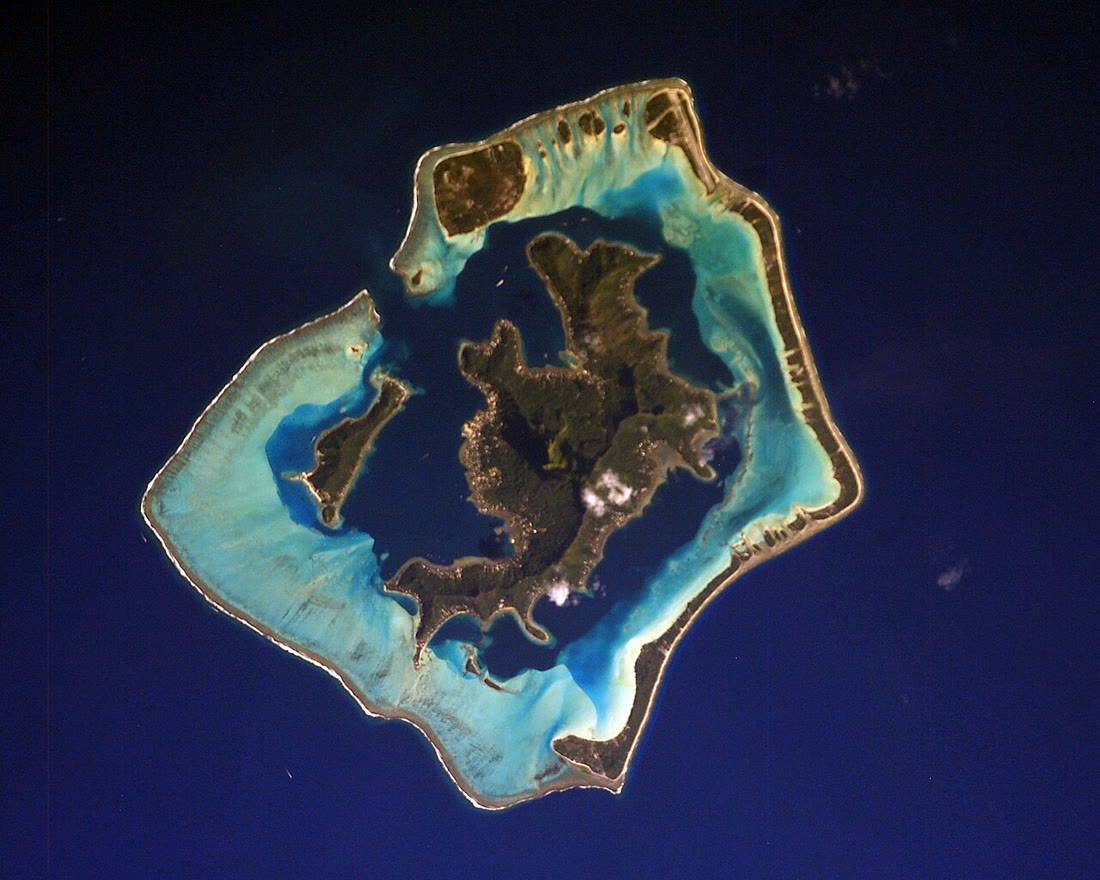
\includegraphics[height=6.9cm]{images/book3/b1-bora-bora.jpg}};
\end{tikzpicture}

{\small 左：三类珊瑚礁的剖面示意（示意图，
竖直比例严重夸大），按达尔文的解释绘制：(a)~
环绕火山岛的裙礁；(b)~岛屿已下沉，礁体向上生长，
已成为与岸线之间隔着泻湖的堡礁；(c)~
岛屿已沉没至视线以下，礁体成为环绕泻湖的环礁，泻湖底部铺有
碳酸盐沉积物。右：博拉博拉岛，为一座火山岛，位于
由堡礁环绕的泻湖之中，礁上有低矮岛屿。该照片由宇航员
于 2003 年 3 月 19 日自国际空间站拍摄（NASA，公有领域，经由
维基共享资源）。}
\label{fig:b1:chemical-biogenic-sediments:reefs}
\end{omfigure}
% ledger: darwin:reefs, commons:bora-bora

\begin{history}[沉降基底上的礁，1837--1842]
在\emph{小猎犬号}的航行途中，查尔斯·达尔文航行于
太平洋与印度洋的礁群之间。他由一个事实出发推断：造礁珊瑚在通常情况下，
通常不能在深于 20 至 30 英寻（约 37 至 \qty{55}{m}）的水域中繁盛。
然而堡礁与环礁却从深水中拔起，远低于这一界限。它们的
基底，他认为，必定曾经下沉，且下沉得足够缓慢，使珊瑚能
借向上生长而保持礁顶位于水面：环绕火山岛的裙礁
随岛屿在其内侧下沉而变为堡礁，
岛屿消失时则变为环礁。他于 1837 年 5 月 31 日在
伦敦地质学会宣读这一理论，并于 1842 年出版 \emph{The Structure and
Distribution of Coral Reefs} 一书，附有一幅将世界上所有礁体
按三种类型分列的地图。海洋岛屿为何下沉、下沉多少，
取决于其下方板块的冷却，将在本科二年级分册中讨论。
\end{history}
% ledger: darwin:reefs

礁只有在其礁顶仍处于造礁生物所栖息的浅水中时才能存活。
海平面会变化，基底也可能下沉；真正起作用的是二者之和，
即相对海平面的上升。

\begin{proposition}[跟上或淹没]\label{prop:b1:chemical-biogenic-sediments:keep-up}
设礁顶位于海平面以下深度 $D_0$ 处，礁体以
速率 $a$ 向上生长，相对海平面以速率 $r$ 上升，二者均为
常数。则经过时间 $t$ 后，礁体上方的水深为
\[
D(t) = D_0 + (r - a)\,t .
\]
若 $a \ge r$，则礁体能跟上海平面（当 $a > r$ 时，礁顶达到
水面，此后只能向侧方生长）；若 $a < r$，则礁体跟不上海平面，
若其造礁生物不能生活在深于 $D_{\max}$ 的水中，则礁体将在
经过时间 $(D_{\max} - D_0)/(r - a)$ 后被淹没。
\end{proposition}

\begin{proof}
自地基上的一个固定标记起向上量取高度。礁顶
位于 $h_0 + a t$ 处，海面位于 $s_0 + r t$ 处，
故礁顶上方的水深为 $D = (s_0 - h_0) + (r - a)t = D_0 + (r-a)t$。当 $a > r$ 时，$D$
在 $t = D_0/(a-r)$ 时减为零，礁体无法再生长到海面以上。若
$a < r$，则 $D$ 线性增长，达到 $D_{\max}$ 的时刻满足 $(r-a)t = D_{\max} -
D_0$。
\end{proof}

礁顶被淹没后，礁体并非立即死亡，但光线变暗、
造礁生物更替、\omterm{def:b1:chemical-biogenic-sediments:factory}{碳酸盐工厂}减速，因此开始落后的礁体会进一步落后：
淹没的礁体与台地，顶部覆有深水沉积物，
在许多大洋岛屿的斜坡上均有发现，
在岩石记录中也可见到。

经过数百万年，\omterm{def:b1:chemical-biogenic-sediments:factory}{碳酸盐工厂}建造出\omterm{def:b1:chemical-biogenic-sediments:reef}{碳酸盐台地}，
即厚层的浅水碳酸盐岩体，随基底沉降而不断增厚。常见两种形态
（见下图）。\emph{镶边陆棚}的顶面平坦，
在其边缘，由礁体与\omterm{def:b1:chemical-biogenic-sediments:reef}{鲕粒}滩构成的镶边保护着顶面，镶边可以
消减波浪；镶边之后是平静的石灰泥泻湖，前方则是
陡坡，从镶边脱落的岩块和碎屑沿此坡落入盆地。
\emph{缓坡}自海岸向盆地极缓倾斜，中间无断折：\omterm{def:b1:chemical-biogenic-sediments:reef}{鲕粒}滩与贝壳滩位于波浪搅动海底之处，
其次是被风暴搬走的贝壳碎屑层，再往下是
波浪所不及的石灰泥。镶边陆棚主要由镶边向上和向外生长，缓坡则
随海平面升降，使沉积带向岸或向海迁移。

\begin{omfigure}
\begin{tikzpicture}[font=\footnotesize, >={Stealth[length=4pt]}]
% (a) rimmed shelf and (b) ramp, schematic cross-sections
\begin{scope}
  \fill[omSea] (0,0.2) rectangle (7.2,2.0);
  \fill[lith limestone, draw=black!60] (0,0) -- (0,1.55) -- (4.3,1.55) -- (4.5,1.75) -- (4.9,1.75) -- (5.1,1.5) -- (6.4,0.35) -- (7.2,0.3) -- (7.2,0) -- cycle;
  \fill[lith reef limestone, draw=black!70] (4.3,1.55) -- (4.5,1.75) -- (4.9,1.75) -- (5.1,1.5) -- (4.8,1.05) -- (4.3,1.05) -- cycle;
  \draw[omSea!60!black] (0,2.0) -- (7.2,2.0);
  \node at (2.1,1.78) {泻湖：石灰泥};
  \node[anchor=south, align=center, font=\scriptsize] at (4.7,2.05) {礁缘与 \\ 鲕粒滩};
  \node[anchor=west, font=\scriptsize] at (5.6,1.2) {斜坡：碎屑};
  \node[font=\scriptsize] at (6.75,0.75) {盆地};
  \node at (3.6,-0.35) {(a) 镶边陆棚};
\end{scope}
\begin{scope}[xshift=8.0cm]
  \fill[omSea] (0,0.2) rectangle (7.2,2.0);
  \fill[lith limestone, draw=black!60] (0,0) -- (0,1.85) -- (7.2,0.55) -- (7.2,0) -- cycle;
  \draw[omSea!60!black] (0,2.0) -- (7.2,2.0);
  \draw[densely dashed, black!50] (0,1.6) -- (7.2,1.6) node[pos=1, anchor=south east, font=\scriptsize, inner sep=1pt] {晴天波浪可及};
  \draw[densely dashed, black!50] (0,1.0) -- (7.2,1.0) node[pos=1, anchor=south east, font=\scriptsize, inner sep=1pt] {风暴波浪可及};
  \node[anchor=south, font=\scriptsize] at (0.9,2.05) {鲕粒滩};
  \node[anchor=south, font=\scriptsize] at (3.4,2.05) {风暴贝壳层};
  \node[anchor=south, font=\scriptsize] at (6.1,2.05) {石灰泥};
  \node at (3.6,-0.35) {(b) 缓坡};
\end{scope}
\end{tikzpicture}

{\small \omterm{def:b1:chemical-biogenic-sediments:reef}{碳酸盐台地}的两种形态（示意图，坡度大幅
夸大）。(a)~镶边陆棚：边缘的礁体与\omterm{def:b1:chemical-biogenic-sediments:reef}{鲕粒}滩消减波浪，
其后为平静的石灰泥泻湖，从镶边脱落的碎屑
沿斜坡滑落至盆地。(b)~缓坡自海岸向盆地极缓倾斜，
沉积物按波浪所能及的深度\omterm{def:b1:clastic-sediments:sorting}{分选}。}
\label{fig:b1:chemical-biogenic-sediments:platforms}
\end{omfigure}

\section{远洋软泥与碳酸盐补偿深度}\label{sec:b1:chemical-biogenic-sediments:oozes}

远离陆地的海底几乎得不到来自大陆的物质，只有
最细的风成尘埃。落到海底的反而是
在上方数千米处日照水层中生活过的浮游生物骨骼：颗石藻的
方解石板片、有孔虫的壳、硅藻的蛋白石质硅壳，
以及放射虫的骨骼
（图见后文）。颗石的长期沉降
落到海底，是形成白垩以及全球大部分
石灰岩的主要过程。
% ledger: nasa:coccoliths-b3, og:carbonates

\begin{definition}[钙质软泥、硅质软泥]\label{def:b1:chemical-biogenic-sediments:ooze}
软泥是细粒的远洋沉积物，沉积于开阔大洋中，
主要由浮游生物的骨骼构成。骨骼为碳酸钙时，
称为\emph{钙质软泥}\index{钙质软泥}，主要为颗石与有孔虫；
骨骼为蛋白石、即水合无定形二氧化硅时，
称为\emph{硅质软泥}\index{硅质软泥}，
主要为硅藻与放射虫。
\end{definition}
% ledger: og:carbonates

\omterm{def:b1:chemical-biogenic-sediments:ooze}{钙质软泥}覆盖了世界海底的约一半，但只限于
某一深度以上：在约 \qty{4500}{m} 以下便消失。贝壳并未停止下沉，
而是在此溶解。深海寒冷、压强高，方解石的溶解度
随深度增大，主要由于压强；水中碳酸根离子的浓度
一般随深度减小（这些平衡的化学原理可参见化学教材）。
在某一深度以下，深层水对方解石未饱和，
到达海底的贝壳埋藏越深，
溶解得越快。
% ledger: britannica:ccd, slotnick:ccd-definitions

\begin{omfigure}
\begin{tikzpicture}
\node[inner sep=0] (a) at (0,0) {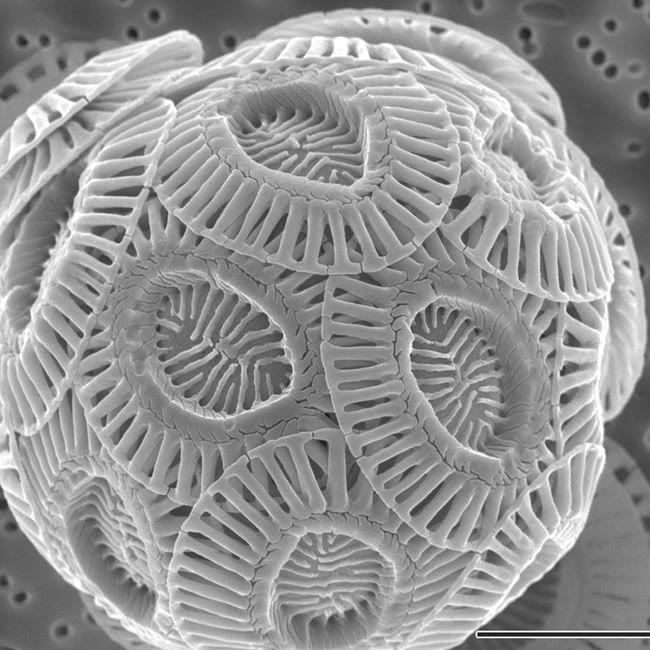
\includegraphics[height=4.3cm]{images/book3/b1-coccolithophore.jpg}};
\node[inner sep=0, anchor=west] (b) at ([xshift=0.25cm]a.east) {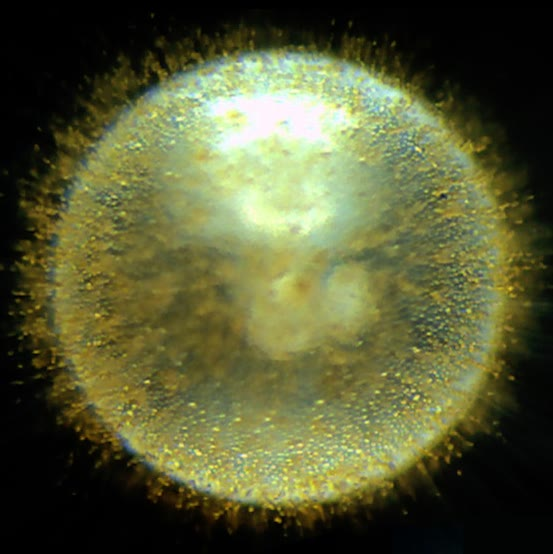
\includegraphics[height=4.3cm]{images/book3/b1-orbulina.jpg}};
\node[inner sep=0, anchor=west] (c) at ([xshift=0.25cm]b.east) {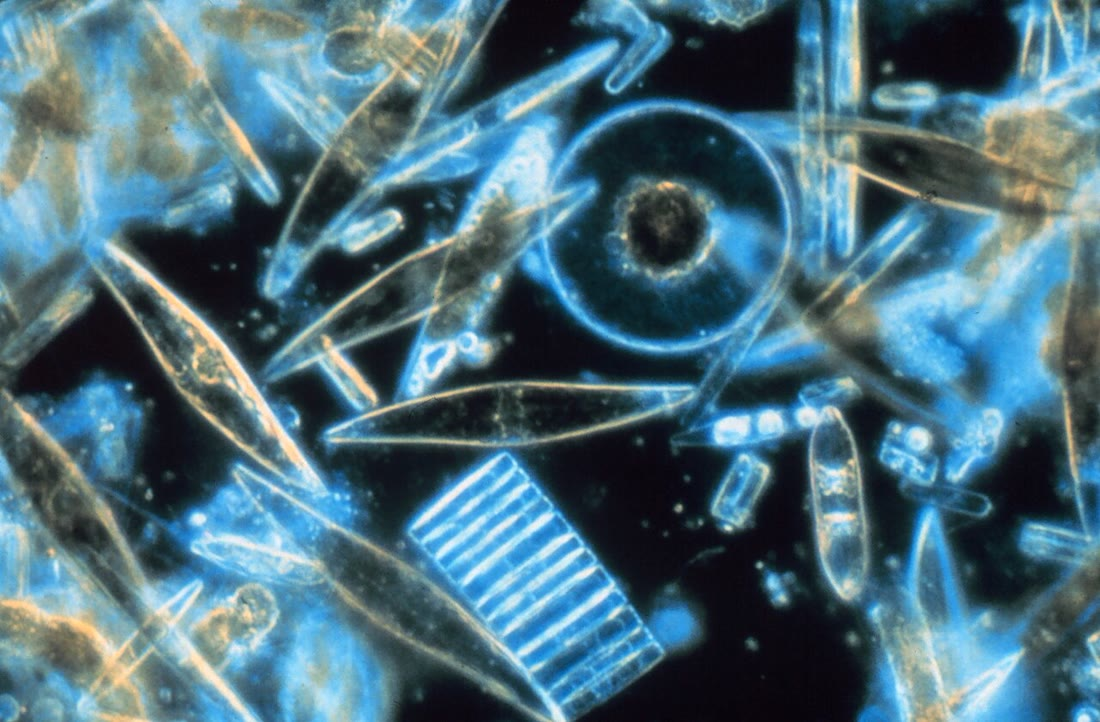
\includegraphics[height=4.3cm]{images/book3/b1-diatoms.jpg}};
\node[font=\footnotesize, anchor=north] at (a.south) {(a) 颗石藻};
\node[font=\footnotesize, anchor=north] at (b.south) {(b) 有孔虫};
\node[font=\footnotesize, anchor=north] at (c.south) {(c) 硅藻};
\end{tikzpicture}

{\small 形成软泥的生物。(a)~\emph{Emiliania huxleyi}的单个细胞，
外被颗石，其方解石板片（扫描电子显微镜；
Alison R.~Taylor，University of North Carolina Wilmington，CC~BY~2.5，经由
维基共享资源。(b)~活的浮游有孔虫，\emph{Orbulina
universa}，其方解石壳周围有刺（光学显微镜；H.~Takagi
等合著者，2019，CC~BY~4.0，经由维基共享资源）。(c)~活的硅藻
取自南极洲麦克默多海峡的海冰，各自包在蛋白石质硅壳中
（光学显微镜；Gordon T.~泰勒，Stony Brook University，NOAA，公有
领域，经由维基共享资源）。}
\label{fig:b1:chemical-biogenic-sediments:plankton}
\end{omfigure}
% ledger: commons:ehux, commons:orbulina, commons:diatoms-noaa

\begin{definition}[溶跃面，碳酸盐补偿深度]\label{def:b1:chemical-biogenic-sediments:ccd}
\emph{溶跃面}\index{溶跃面}是海洋中的一个深度，在其以下，
海底方解石的溶解首先在沉积物中显现，
且溶解速率急剧增大。\emph{碳酸盐补偿
深度}\index{碳酸盐补偿深度}（CCD）是方解石
的溶解速率恰好等于方解石落到海底速率的深度，
在其以下没有碳酸钙堆积。实际上，它取为表层沉积物的
碳酸钙含量降至 \qty{10}{\%} 以下的深度，
以质量计。
\end{definition}
% ledger: slotnick:ccd-definitions

\omterm{def:b1:chemical-biogenic-sediments:ccd}{碳酸盐补偿深度}（CCD）通常位于\omterm{def:b1:chemical-biogenic-sediments:ccd}{溶跃面}以下数百米处。它并非
固定的水平面：它由供给与溶解之间的平衡决定，因此
位置更深，即浮游生物产生更多碳酸盐、深层水
腐蚀性较弱之处。在大西洋，它比太平洋约深 \qty{500}{m}，
这是碳酸盐供给更多、溶解更慢共同作用的结果；
仅在西太平洋内，
其西北部约位于 \qty{4000}{m}，
中太平洋约位于 \qty{5100}{m}。文石比方解石更易溶，
在更浅的深度即已溶解。在地质时间尺度上，
供给、生产力和溶解方面的变化使 CCD 移动了
\qty{2000}{m} 以上。
% ledger: slotnick:ccd-definitions, britannica:ccd, zhang:ccd-west-pacific

\begin{method}[确定溶跃面与 CCD 的位置]\label{met:b1:chemical-biogenic-sediments:ccd}
\begin{enumerate}
  \item 在同一区域内不同水深处采集表层数厘米厚的沉积物，
        站点须足够远离陆地和上升流，使黏土或蛋白石的稀释
        作用足够小。
  \item 测定每个样品中 \ce{CaCO3} 的质量百分数，并将其
        与水深作图。
  \item \omterm{def:b1:chemical-biogenic-sediments:ccd}{溶跃面}是含量开始陡降的深度，
        也是壳体首次出现溶解迹象的深度（破碎、
        被蚀刻的有孔虫）。
  \item CCD 是含量降至 \qty{10}{\%} 的深度：由
        两侧相邻两个样品之间线性插值读出。
\end{enumerate}
\end{method}

在洋中脊的侧翼，海底靠近
轴部处年轻且较浅，随年龄增长并远离轴部而下沉。诞生于 CCD 以上的一块海底
堆积\omterm{def:b1:chemical-biogenic-sediments:ooze}{钙质软泥}，直至下沉到 CCD 以下；此后它
只接收不会溶解的物质：从上空沉降的尘埃、铁和
锰的氧化物以及鱼的牙齿。这种缓慢形成的棕色沉积物即是
深海盆地中的红黏土。

\begin{proposition}[穿越 CCD]\label{prop:b1:chemical-biogenic-sediments:flank}
设年龄为 $t$ 的海底位于深度 $d(t) = d_r + C\sqrt t$
（见\cref{thm:b1:rifts-ridges-margins:depth-age}），洋脊轴部位于深度 $d_r$
浅于一个保持不变的\omterm{def:b1:chemical-biogenic-sediments:ccd}{碳酸盐补偿深度} $z_c$。则
海底穿越 CCD 的年龄为
\[
t_c = \left(\frac{z_c - d_r}{C}\right)^2 ,
\]
年龄 $t > t_c$ 的站点自下而上依次承载：火山\omterm{def:b1:layered-earth:layers}{地壳}、
时间 $t_c$ 内沉积的\omterm{def:b1:chemical-biogenic-sediments:ooze}{钙质软泥}，以及在
时间 $t - t_c$ 内沉积的红黏土。
\end{proposition}

\begin{proof}
深度 $d(t)$ 随 $t$ 增大，由 $d(t_c) = z_c$ 得 $C\sqrt{t_c} =
z_c - d_r$，从而得 $t_c$。在 $t_c$ 之前，海底位于 CCD 以上，此处
方解石落下的速率快于溶解，软泥得以堆积；在 $t_c$ 之后，它
位于其下，此处无碳酸盐堆积，只有不溶的黏土
被加入。软泥一旦被黏土掩埋，便免受上方腐蚀性海水的侵蚀，
因此各层的顺序与时间顺序一致。
\end{proof}

取 $d = 2500 + 350\sqrt t$（深度以米计，$t$ 以百万年计），CCD 位于
\qty{4500}{m} 处，穿越它的年龄为 $(2000/350)^2 = \qty{32.7}{Ma}$；若
\omterm{def:b1:plate-kinematics:spreading-rate}{半扩张速率}为 \qty{25}{mm} 每年，则此处距轴部 \qty{816}{km}
（见下图）。钻探古老的洋底时，
一再发现这一层序：玄武岩、\omterm{def:b1:chemical-biogenic-sediments:ooze}{钙质软泥}或白垩，
其上为红黏土，它记录了海底沿侧翼下沉的历程。板块
此后移到赤道附近一条高生产力带之下，黏土
可被一层新的软泥覆盖，岩芯正是借此记录了
板块的运动以及 CCD 的深度。
% ledger: parsons:plate-model

\begin{omfigure}
\begin{tikzpicture}[font=\footnotesize]
\begin{axis}[width=11cm, height=5.6cm, xmin=0, xmax=1750, ymin=2000, ymax=6200, y dir=reverse,
    xlabel={距洋脊轴的距离（km），半扩张速率 \qty{25}{mm.\text{年}^{-1}}},
    ylabel={深度（m）}, ytick={2000,3000,...,6000},
    axis on top, clip=false]
  % sea water above the floor
  \addplot[fill=omSea, draw=none] table[x=x_km, y=depth] {figdata/out/bachelor-1-ccd_flank-profile.dat} -- (axis cs:1750,2000) -- (axis cs:0,2000) -- cycle;
  % floor: ooze-covered above the CCD, red clay below
  \addplot[very thick, draw=omLithLime!70!black, restrict x to domain=0:816.3] table[x=x_km, y=depth] {figdata/out/bachelor-1-ccd_flank-profile.dat};
  \addplot[very thick, draw=brown!70!black, restrict x to domain=816.3:1750] table[x=x_km, y=depth] {figdata/out/bachelor-1-ccd_flank-profile.dat};
  \draw[thick, omThm, densely dashed] (axis cs:0,4500) -- (axis cs:1750,4500) node[pos=0.99, anchor=north east, inner sep=1.5pt] {CCD，\qty{4500}{m}};
  \draw[black!60, dotted, thick] (axis cs:0,4050) -- (axis cs:1750,4050) node[pos=0.99, anchor=south east, inner sep=1.5pt] {溶跃面（示意）};
  \fill[omThm] (axis cs:816.3,4500) circle[radius=2pt];
  \node[anchor=north east, align=right] at (axis cs:790,4620) {海底穿越 CCD\\ 于 \qty{32.7}{Ma}，距轴 \qty{816}{km}};
  \node[anchor=north, align=center, omLithLime!40!black] at (axis cs:520,2750) {钙质软泥 \\ 堆积};
  \node[anchor=north west, align=left, brown!60!black] at (axis cs:1000,5180) {红黏土覆盖 \\ 被掩埋的软泥};
\end{axis}
% sediment column at the site 1500 km from the axis (60 Myr), schematic
\begin{scope}[xshift=10.6cm, yshift=0.4cm]
  \draw[lith basalt] (0,0) rectangle (0.9,1.0);
  \draw[lith limestone] (0,1.0) rectangle (0.9,2.6);
  \fill[brown!45, draw=black!60] (0,2.6) rectangle (0.9,3.2);
  \node[anchor=west, align=left, font=\scriptsize] at (1.0,0.5) {玄武质地壳};
  \node[anchor=west, align=left, font=\scriptsize] at (1.0,1.8) {钙质软泥 \\ （0 至 \qty{32.7}{Ma}）};
  \node[anchor=west, align=left, font=\scriptsize] at (1.0,2.9) {红黏土};
  \node[anchor=south, font=\scriptsize, align=center] at (0.9,3.3) {距轴 \qty{1500}{km} 处的剖面柱 \\ （示意）};
\end{scope}
\end{tikzpicture}

{\small 洋脊侧翼的远洋沉积物。海底深度随年龄增加，
依\omterm{thm:b1:rifts-ridges-margins:depth-age}{深度–年龄关系} $d = 2500 + 350\sqrt t$ 给出，并以
每年 \qty{25}{mm} 的速度远离洋脊轴；\omterm{def:b1:chemical-biogenic-sediments:ccd}{碳酸盐补偿深度}（此处取
\qty{4500}{m}）以上沉积\omterm{def:b1:chemical-biogenic-sediments:ooze}{钙质软泥}，以下则只有红黏土。远离轴线的站点
自下而上依次为玄武岩、软泥和红黏土（见右侧剖面柱，
厚度为示意）。\omterm{def:b1:chemical-biogenic-sediments:ccd}{溶跃面}画于\omterm{def:b1:chemical-biogenic-sediments:ccd}{碳酸盐补偿深度}之上数百米处，
标示溶解开始显现的位置。}
\label{fig:b1:chemical-biogenic-sediments:flank}
\end{omfigure}
% computed in figdata/bachelor-1/ccd_flank.py; ledger: parsons:plate-model, britannica:ccd, slotnick:ccd-definitions

\section{硅质软泥与燧石}\label{sec:b1:chemical-biogenic-sediments:silica}

硅藻是浮游植物中的单细胞藻类，放射虫是浮游动物中的单细胞成员，
二者以蛋白石构建骨骼，其原料取自
海水中溶解的硅酸。与表层海洋的方解石
不同，蛋白石不受过饱和保护：海水在各深度上
对它都未饱和，因此大部分蛋白石在生物死亡后
即溶解，先在下沉途中，随后在海底溶解。全球海洋浮游生物每年构建进蛋白石的硅共 255~太摩尔，
其中仅
约 9.2 被永久埋入沉积物，保存率为
\qty{3.6}{\%}。由河流带入海洋的一个硅原子被浮游生物摄取，
并再释放约 16 次，之后才被埋藏，它在海洋中停留
约 \num{8000} 年。
% ledger: treguer:silica

因此\omterm{def:b1:chemical-biogenic-sediments:ooze}{硅质软泥}形成于蛋白石产量极高、
以致即使只有 \qty{3.6}{\%} 被保存也能积累，且鲜有其他沉积物稀释之处，大致在
南大洋周围、北太平洋、太平洋赤道沿线，以及
大陆边缘，即富含营养盐的深层水上升至
表层的海域（见\cref{ch:b1:ocean-circulation}）。它们也在\omterm{def:b1:chemical-biogenic-sediments:ccd}{碳酸盐补偿深度}以下占主导，
即高产水体之下，那里与之同沉的方解石已溶解。
% ledger: treguer:silica, og:carbonates

\begin{definition}[燧石]\label{def:b1:chemical-biogenic-sediments:chert}
\emph{燧石}\index{燧石}是由微晶石英构成的坚硬致密的沉积岩，
大多由埋藏后溶解并再结晶的生物成因蛋白石形成，
常以层状产出，多来自\omterm{def:b1:chemical-biogenic-sediments:ooze}{硅质软泥}，
或以结核状产出，其中以白垩中的火石最为人所知。
\end{definition}
% ledger: og:carbonates

未经再结晶的硅藻软泥变为硅藻土，
一种轻质、白色、多孔的岩石，几乎是纯蛋白石。随埋藏和时间推移，蛋白石转变为
其他形式的二氧化硅，最终变为石英，二氧化硅发生迁移：它
例如离开白垩，并沿某些
岩层聚集成火石结核。这一过程属于成岩作用（见\cref{ch:b1:diagenesis-basins}）。

\section{蒸发岩}\label{sec:b1:chemical-biogenic-sediments:evaporites}

若某一海水水体因蒸发失水多于获得的水量，
其中的盐分不断浓缩，直至依次沉淀。海水的
主要离子组成在各大洋中相同
（见\cref{tab:b1:chemical-biogenic-sediments:seawater}）。

\begin{table}[htbp]
\centering\small
\begin{tabular}{@{}lrrr@{}}
\hline
离子 & 海盐质量分数 & \si{g} 每 \si{kg} 海水 & \si{mmol} 每 \si{kg} \\
\hline
氯离子 \ce{Cl-} & 0.5503 & 19.353 & 545.9 \\
钠离子 \ce{Na+} & 0.3066 & 10.781 & 469.0 \\
硫酸根 \ce{SO4^2-} & 0.0771 & 2.712 & 28.2 \\
镁离子 \ce{Mg^2+} & 0.0365 & 1.284 & 52.8 \\
钙离子 \ce{Ca^2+} & 0.0117 & 0.412 & 10.3 \\
钾离子 \ce{K+} & 0.0113 & 0.399 & 10.2 \\
碳酸氢根 \ce{HCO3-} & 0.0030 & 0.105 & 1.72 \\
溴离子 \ce{Br-} & 0.0019 & 0.067 & 0.84 \\
\hline
所有溶质 & 1 & 35.165 & \\
\hline
\end{tabular}
\caption{参考组成海水的主要离子，其盐度为
每千克海水含 \qty{35.165}{g} 盐。氯与
钠占盐质量的 \qty{86}{\%}；碳酸根、锶、硼酸根与
氟则占其余的大部分。}
\label{tab:b1:chemical-biogenic-sediments:seawater}
\end{table}
% ledger: teos10:reference-composition, teos10:reference-salinity (g and mmol computed in evaporation.py)

\begin{definition}[蒸发岩、蒸发序列、萨布哈]\label{def:b1:chemical-biogenic-sediments:evaporite}
\emph{蒸发岩}\index{蒸发岩}是由盐类形成的沉积物或沉积岩，
这些盐类由经蒸发浓缩的天然卤水沉淀而成，主要为石膏
\ce{CaSO4.2H2O}、硬石膏 \ce{CaSO4}、岩盐 \ce{NaCl}，以及钾盐和
镁盐。\emph{蒸发序列}\index{蒸发序列}是蒸发海水时\omterm{def:b1:rock-forming-minerals:mineral}{矿物}的沉淀次序，
溶解度最小者最先沉淀：
依次为碳酸钙、石膏、岩盐，然后是钾盐与镁盐。
\emph{萨布哈}\index{萨布哈}是沿海盐沼，位于
最高潮位或略高于其的水平，其中石膏、硬石膏和岩盐
由浸透沉积物的蒸发卤水在沉积物内生长。
\end{definition}
% ledger: og:carbonates, warren:brine-stages

早在 1849 年，尤西利奥便观察了这一序列，他将一容器海水
蒸干。最精确的测量来自巴哈马的大伊纳瓜岛盐场，
海水在那里被引经一系列
浓度递增的盐池。碳酸钙开始沉淀时，卤水的浓度
为海水的 1.8~倍，石膏为 3.8~倍，岩盐为
10.6~倍；实验室中硫酸镁随后沉淀，约在 70~倍时析出，钾盐则在 90~倍以上析出。
由于先前沉淀的盐类质量可以忽略，
浓缩因子 10.6 意味着 $1/10.6$，
即约 \qty{9}{\%} 的水留存，故岩盐只在
九成的水蒸发掉后才出现（见下图 a 部分）。
卤水随浓缩而变稠，海水的密度为 \qty{1.03}{g.cm^{-3}}，
析出石膏时约为 \num{1.13}，析出岩盐时为 \num{1.22}，
析出苦卤盐时超过 \num{1.30}，它们是最后析出的盐类。
% ledger: warren:brine-stages, mccaffrey:thresholds

每千克海水能提供多少各种盐，可由
\cref{tab:b1:chemical-biogenic-sediments:seawater}，通过统计
先耗尽的离子求出。碳酸钙受碳酸根和碳酸氢根的限制，
为 \qty{1.10}{mmol}，约 \qty{0.11}{g}。石膏占用剩余的钙，
为 \qty{9.18}{mmol}，\qty{1.58}{g}，硫酸根过量。岩盐占用全部的
钠，为 \qty{469}{mmol}，\qty{27.4}{g}，氯离子过量。剩余的
约 \qty{6.3}{g} 的镁、钾、硫酸根、氯离子和溴离子构成
苦卤盐。岩盐占总量的 \qty{78}{\%}：\omterm{def:b1:chemical-biogenic-sediments:evaporite}{蒸发岩}盆地
干涸后，主要是一大块岩盐。
% computed in figdata/bachelor-1/evaporation.py; ledger: teos10:reference-composition, mccaffrey:thresholds

\begin{omfigure}
\begin{tikzpicture}[font=\footnotesize]
\begin{axis}[name=a, width=7.6cm, height=5.6cm, xmode=log, xmin=1, xmax=100, ymin=0, ymax=1.05,
    xlabel={卤水的浓缩倍数}, ylabel={剩余水的比例},
    title={\footnotesize (a) 蒸发序列的起始点}, grid=major, grid style={black!10},
    log ticks with fixed point]
  \addplot[omDef, thick] table[x=CF, y=f_left] {figdata/out/bachelor-1-evaporation-curve.dat};
  \addplot[omThm, only marks, mark=*, mark size=1.8pt] table[x=CF, y=f_left] {figdata/out/bachelor-1-evaporation-steps.dat};
  \node[anchor=south west, font=\scriptsize] at (axis cs:1.8,0.556) {\ce{CaCO3} (1.8)};
  \node[anchor=south west, font=\scriptsize] at (axis cs:3.8,0.263) {石膏 (3.8)};
  \node[anchor=south west, font=\scriptsize] at (axis cs:10.6,0.094) {岩盐 (10.6)};
  \node[anchor=south, font=\scriptsize, align=center] at (axis cs:60,0.16) {Mg、K 盐 \\ (70, 90)};
\end{axis}
\begin{axis}[at={(a.east)}, anchor=west, xshift=1.7cm, width=7.0cm, height=5.6cm,
    ybar, bar width=14pt, ymin=0, ymax=32, xmin=0.4, xmax=4.6,
    xtick={1,2,3,4}, xticklabels={\ce{CaCO3}, 石膏, 岩盐, 苦卤},
    ylabel={每千克海水的克数}, title={\footnotesize (b) 析出的质量},
    nodes near coords, nodes near coords style={font=\scriptsize, /pgf/number format/precision=2},
    every node near coord/.append style={/pgf/number format/fixed}]
  \addplot[fill=omDef!40, draw=omDef] table[x=idx, y=g_per_kg] {figdata/out/bachelor-1-evaporation-masses.dat};
\end{axis}
\end{tikzpicture}

{\small 海水的蒸发。(a)~卤水被浓缩至给定倍数时剩余水的比例，
以及各\omterm{def:b1:rock-forming-minerals:mineral}{矿物}开始析出的点，
分别在大伊纳瓜盐场及实验室中测定（McCaffrey,
Lazar and Holland, 1987）。(b)~每千克海水
蒸干后析出的各\omterm{def:b1:rock-forming-minerals:mineral}{矿物}质量，每种\omterm{def:b1:rock-forming-minerals:mineral}{矿物}取尽限制它的离子，
（石膏计入结晶水，苦卤盐不计结晶水），
依据海水的参考组成计算。}
\label{fig:b1:chemical-biogenic-sediments:evaporation}
\end{omfigure}
% computed in figdata/bachelor-1/evaporation.py; ledger: mccaffrey:thresholds, teos10:reference-composition

由这些质量，一定水体所能留下的盐层厚度
可直接算出。

\begin{proposition}[海水柱中的盐]\label{prop:b1:chemical-biogenic-sediments:column}
高为 $H$、密度为 $\rho_{sw}$ 的海水柱，蒸干后
析出一层密度为 $\rho_x$ 的\omterm{def:b1:rock-forming-minerals:mineral}{矿物}层，其厚度为
\[
h_x = \frac{\rho_{sw}\,H\,m_x}{\rho_x},
\]
其中 $m_x$ 为每单位质量海水析出的该\omterm{def:b1:rock-forming-minerals:mineral}{矿物}质量。
\end{proposition}

\begin{proof}
单位面积的海水柱含有质量为 $\rho_{sw}H$ 的海水，其析出
的\omterm{def:b1:rock-forming-minerals:mineral}{矿物}质量为 $\rho_{sw}Hm_x$。将其铺于同一单位面积，
作为密度为 $\rho_x$ 的一层，其厚度为 $\rho_{sw}Hm_x/\rho_x$。
\end{proof}

取 $\rho_{sw} = \qty{1030}{kg.m^{-3}}$、$m = \qty{27.4}{g.kg^{-1}}$，
以及岩盐的密度 \qty{2170}{kg.m^{-3}}，则高 \qty{1000}{m} 的海水柱
可留下 \qty{13.0}{m} 厚的岩盐；若为石膏，其密度为 \qty{2300}{kg.m^{-3}}，则
可留下 \qty{0.71}{m} 厚的石膏。这就是\omterm{def:b1:chemical-biogenic-sediments:evaporite}{蒸发岩}的厚度问题：
数百米乃至数千米厚的盐层，
无论盆地多深，都不可能是某一次充填后蒸发的残留物。
% computed in figdata/bachelor-1/evaporation.py; ledger: warren:brine-stages, webmineral:evaporites

答案在于一个持续接纳海水的盆地。与海洋
以岩床、浅水海峡或堤坝相隔的盆地，在干旱气候下，
通过整个盆地面积的蒸发失水；海水越过岩床流入以补充，
带入新的盐分，而较重的卤水可能在深处越过岩床流出
（见下图）。卤水的浓缩程度
由这些水流的平衡决定。

\begin{proposition}[有障壁的盆地]\label{prop:b1:chemical-biogenic-sediments:barred}
设面积为 $A$ 的充分混合盆地，单位时间内因净蒸发失去体积为 $EA$ 的水，
以体积流量 $Q_{\mathrm{in}}$ 接纳海水，
并以体积流量 $Q_{\mathrm{out}}$ 向海洋回注卤水，处于
稳态。对于不析出的离子，卤水相对于海水的浓缩
倍数为
\[
k = \frac{Q_{\mathrm{in}}}{Q_{\mathrm{out}}} = \frac{Q_{\mathrm{in}}}{Q_{\mathrm{in}} - EA}
\]
相对于海水而言（体积按等密度计算）。
\end{proposition}

\begin{proof}
稳态下盆地体积不变，因此流入量
与流出量及蒸发量相平衡：$Q_{\mathrm{in}} = Q_{\mathrm{out}} +
EA$。离子以海水的浓度 $c_0$ 进入，仅随卤水流出，
其浓度为 $c$；因其不析出，盆地中的质量
稳定的条件为 $Q_{\mathrm{in}}c_0 = Q_{\mathrm{out}}c$。由此 $c/c_0 =
Q_{\mathrm{in}}/Q_{\mathrm{out}}$，代入 $Q_{\mathrm{out}}$ 得到
第二种形式。
\end{proof}

盆地析出何种\omterm{def:b1:rock-forming-minerals:mineral}{矿物}，由流出量决定。若流回海洋的卤水超过流入量的
十分之一，则 $k$ 保持在 10.6 以下，盆地只析出
碳酸盐和石膏，而绝不析出岩盐；若流出量更小，
卤水达到岩盐饱和，盆地被盐充填；若海峡
完全封闭，盆地干涸，水位以速率 $E$ 下降。

\begin{omfigure}
\begin{tikzpicture}[font=\footnotesize, >={Stealth[length=4pt]}]
% barred evaporite basin (schematic)
\fill[omSea] (0,1.0) rectangle (3.2,3.0);
\fill[omSea!70!yellow!40] (3.6,0.6) rectangle (11.2,3.0);
\fill[omSea] (3.0,2.45) rectangle (3.8,3.0);
\draw[lith shale] (0,0) -- (0,1.0) -- (2.6,1.0) -- (3.2,2.4) -- (3.6,2.45) -- (4.4,0.6) -- (10.2,0.6) -- (11.2,2.2) -- (11.2,0) -- cycle;
\draw[lith evaporite] (4.25,0.95) -- (4.4,0.6) -- (10.2,0.6) -- (10.41,0.95) -- cycle;
\fill[omLithGranite!50, draw=black!50] (5.6,0.95) rectangle (9.0,1.35);
\draw[omSea!60!black] (0,3.0) -- (11.2,3.0);
\draw[->, thick, omDef] (1.6,2.75) -- (4.6,2.75) node[right] {海水流入};
\draw[->, thick, omThm, densely dashed] (4.6,1.5) .. controls (4.1,2.35) and (3.8,2.57) .. (3.1,2.57) .. controls (2.6,2.57) and (2.3,2.2) .. (2.1,1.7) node[anchor=north east, inner sep=1pt] {卤水流出};
\foreach \x in {6.0,7.4,8.8,10.2} {\draw[->, black!60] (\x,3.1) -- (\x,3.7);}
\node[anchor=south] at (8.1,3.7) {盆地表面蒸发};
\node at (0.8,2.15) {海洋};
\node[anchor=south] at (3.4,3.0) {岩床};
\node[anchor=north, fill=white, inner sep=1pt] at (7.3,0.55) {石膏和硬石膏};
\node at (7.3,1.15) {岩盐};
\node at (7.3,2.2) {高密度卤水};
\end{tikzpicture}

{\small 有坎蒸发盆地（示意）：海水越过岩床流入，
以补充盆地蒸发掉的水；高密度卤水下沉，部分
卤水在深处流回大洋。流出量越小，卤水越
浓缩；此时卤水已越过岩盐饱和点，岩盐
覆盖在早先形成的石膏之上。}
\label{fig:b1:chemical-biogenic-sediments:barred}
\end{omfigure}

世界上最大的年轻\omterm{def:b1:chemical-biogenic-sediments:evaporite}{蒸发岩}位于地中海
海底之下。距今597万至533万年前，即墨西拿阶，
地中海与大西洋之间的水体交换受到限制，
深盆地中沉积了厚达\qty{2}{km}的\omterm{def:b1:chemical-biogenic-sediments:evaporite}{蒸发岩}，其中
岩盐主要形成于距今560万至555万年前的短暂时段。
其形成过程至今仍有争议。一种模型认为，海洋大部分被切断，其
水位下降约\qty{1500}{m}，深盆地变为盐湖，河流
在干涸的边缘切出深谷；另一些模型则认为盆地保持
连通且充满水，即大尺度的有坎盆地。两种模型都必须解释
千米厚的盐层，这是一次海水充注绝不可能形成的。
% ledger: vasiliev:msc

\section{练习}

\begin{exercise}[$\star$]\label{exo:b1:chemical-biogenic-sediments:1}
参考成分的海水每千克含盐\qty{35.165}{g}，其中
氯、钠、硫酸根和镁的质量分数分别为
0.5503、0.3066、0.0771 和 0.0365。求每千克海水中各离子的质量，
以及钠和氯合计占盐的比例。
% ledger: teos10:reference-composition, teos10:reference-salinity
\end{exercise}

\begin{exercise}[$\star$]\label{exo:b1:chemical-biogenic-sediments:2}
碳酸钙、石膏、岩盐和硫酸镁在海水浓缩至
1.8、3.8、10.6 和 70 倍时开始从海水中析出。对每种\omterm{def:b1:rock-forming-minerals:mineral}{矿物}，求
剩余原始水量的比例和已蒸发水量的比例。
% ledger: mccaffrey:thresholds
\end{exercise}

\begin{exercise}[$\star$]\label{exo:b1:chemical-biogenic-sediments:3}
在以\emph{Acropora}为优势种的礁上，碳酸盐收支为\qty{8.4}{kg}
\ce{CaCO3}（每平方米每年），礁体每年生长\qty{4.2}{mm}。
(a)~由\cref{prop:b1:chemical-biogenic-sediments:accretion}，求礁体的
干体积密度。(b)~若颗粒为文石，
密度为\qty{2.93}{g.cm^{-3}}；若为方解石，密度为
\qty{2.71}{g.cm^{-3}}，则其孔隙度分别为多少？(c)~在相同体积密度下，
平均收支为\qty{3.7}{kg.m^{-2}.\text{年}^{-1}}的礁体将以多快的速度生长？
% ledger: perry:chagos, webmineral:polymorphs, hom:calcite
\end{exercise}

\begin{exercise}[$\star$]\label{exo:b1:chemical-biogenic-sediments:4}
洋底某一区域的表层沉积物中，\ce{CaCO3}的重量百分数如下：
\qty{3000}{m}处为88，\qty{3500}{m}处为85，
\qty{4000}{m}处为80，\qty{4300}{m}处为62，\qty{4500}{m}处为35，\qty{4700}{m}处为12，\qty{4800}{m}处为6，
\qty{5000}{m}处为2。依据
\cref{met:b1:chemical-biogenic-sediments:ccd}，确定\omterm{def:b1:chemical-biogenic-sediments:ccd}{溶跃面}与 CCD 的位置。
\end{exercise}

\begin{exercise}[$\star\star$]\label{exo:b1:chemical-biogenic-sediments:5}
(a)~写出由钙离子与碳酸氢根离子沉淀碳酸钙的配平方程式，
并计算每千克沉积的\ce{CaCO3}所释放的
二氧化碳质量（摩尔质量分别为\qty{100.09}{g.mol^{-1}}
和\qty{44.01}{g.mol^{-1}}）。(b)~礁体收支为
\qty{3.7}{kg.m^{-2}.\text{年}^{-1}}时，按此方程每平方米每年释放的
二氧化碳量为多少？(c)~为何将溶解态碳转化为岩石的礁体
会释放二氧化碳？
% ledger: perry:chagos
\end{exercise}

\begin{exercise}[$\star\star$]\label{exo:b1:chemical-biogenic-sediments:6}
取洋底深度 $d = 2500 + 350\sqrt t$（单位为米，$t$ 以
百万年计），自洋脊以\omterm{def:b1:plate-kinematics:spreading-rate}{半扩张速率}\qty{25}{mm}
每年扩张。(a)~洋底在何年龄、距轴多远处穿越
\qty{4500}{m}处的 CCD？(b)~对于 \qty{5100}{m} 处的 CCD，
即中太平洋的情形。(c)~年龄为\qty{60}{Ma}的洋底，在
两种情况下各接收了多长时间的红黏土？
% ledger: parsons:plate-model, zhang:ccd-west-pacific
\end{exercise}

\begin{exercise}[$\star\star$]\label{exo:b1:chemical-biogenic-sediments:7}
礁体每年生长\qty{4.2}{mm}。(a)~它能否跟上相对
海平面每年\qty{3}{mm}的上升？(b)~其顶部位于海面以下\qty{2}{m}处，
当相对上升速率变为每年\qty{10}{mm}时，若造礁者不能
生活在深于\qty{50}{m}处，则需多久才会被淹没？
(c)~为何它实际上可能更早被淹没？
% ledger: perry:chagos
\end{exercise}

\begin{exercise}[$\star\star$]\label{exo:b1:chemical-biogenic-sediments:8}
埋藏于数百米沉积物之下的石膏\ce{CaSO4.2H2O}
（摩尔质量\qty{172.17}{g.mol^{-1}}，密度\qty{2.30}{g.cm^{-3}}）失去水分，
转变为硬石膏\ce{CaSO4}（摩尔质量\qty{136.14}{g.mol^{-1}}，密度
\qty{2.97}{g.cm^{-3}}）。(a)~写出反应式。(b)~求两种\omterm{def:b1:rock-forming-minerals:mineral}{矿物}的
摩尔体积及固体的体积变化。(c)~石膏质量中有多大比例
以水的形式离开？这些水能对周围的岩石产生什么
作用？
% ledger: webmineral:evaporites
\end{exercise}

\begin{exercise}[$\star\star$]\label{exo:b1:chemical-biogenic-sediments:9}
世界大洋的浮游生物每年将 255 太摩尔的硅
转化为蛋白石，其中 9.2 太摩尔被埋藏。(a)~求被保存的比例与
溶解的比例。(b)~为何\omterm{def:b1:chemical-biogenic-sediments:ooze}{硅质软泥}仍能形成，又形成于何处？(c)~
为何沉积物中的硅藻记录是对
水中实际生存硅藻的有偏反映？
% ledger: treguer:silica
\end{exercise}

\begin{exercise}[$\star\star\star$]\label{exo:b1:chemical-biogenic-sediments:10}
面积为\qty{10000}{km^2}的有坎盆地，每年因净蒸发损失\qty{1.5}{m}
厚的水。(a)~求每年蒸发的水体积。(b)~依据
\cref{prop:b1:chemical-biogenic-sediments:barred}，求卤水的浓缩倍数，
当每年越过岩床的入流量为\qty{1.8e10}{m^3}时，
以及为\qty{1.575e10}{m^3}时，
两种情况下各有哪些\omterm{def:b1:rock-forming-minerals:mineral}{矿物}可以析出？(c)~入流量不超过多少时，该盆地沉积岩盐？
% ledger: mccaffrey:thresholds
\end{exercise}

\begin{exercise}[$\star\star\star$]\label{exo:b1:chemical-biogenic-sediments:11}
海水每千克含\qty{0.0673}{g}溴。岩盐析出时，
其吸收的溴与卤水中的浓度成正比：
岩盐中的溴含量为卤水的 $D = 0.032$ 倍。
(a)~求卤水中的溴含量（单位为毫克每千克）以及首批岩盐中的溴含量，
当卤水浓度为海水的 10.6~倍时。
(b)~卤水浓度达到海水的 30~倍时，求同样的量。(c)~岩盐几乎不从卤水中带走溴：
为什么？(d)~在厚层岩盐中，
溴含量向上升高，随后突然回落。
盆地发生了什么变化？
% ledger: teos10:reference-composition, mccaffrey:dbr, mccaffrey:thresholds
\end{exercise}

\begin{exercise}[$\star\star\star$]\label{exo:b1:chemical-biogenic-sediments:12}
某地点位于洋脊侧翼，其深度为 $d = 2500 + 350\sqrt t$，现今年龄为
\qty{70}{Ma}。设\omterm{def:b1:chemical-biogenic-sediments:ooze}{钙质软泥}以每千年\qty{2}{cm}的速率堆积于
\omterm{def:b1:chemical-biogenic-sediments:ccd}{碳酸盐补偿深度}以上，红粘土以每千年\qty{1}{mm}的速率堆积于
\omterm{def:b1:chemical-biogenic-sediments:ccd}{碳酸盐补偿深度}以下，并忽略压实作用。(a)~求该地点软泥与红粘土的
厚度，\omterm{def:b1:chemical-biogenic-sediments:ccd}{碳酸盐补偿深度}为\qty{4500}{m}时。(b)~\omterm{def:b1:chemical-biogenic-sediments:ccd}{碳酸盐补偿深度}
再加深\qty{500}{m}（如大西洋的情况），求同样的量。(c)~该地点的一根岩芯
显示出红粘土中有一薄层软泥。给出两种可能的解释。
% ledger: parsons:plate-model, britannica:ccd
\end{exercise}

\section{问题：来自消失之海的盐}

\begin{problem}[{周末问题——形成一个盐盆需要多少海水，
以及需要多长时间}]
\label{pb:b1:chemical-biogenic-sediments:1}
% values: calc/ch22.py; the basin, its area, inflow and evaporation are invented
一个面积为 $A = \qty{1.0e5}{km^2}$、深 \qty{1000}{m} 的内陆海，
通过一道位于浅岩床上的海峡与大洋相连。其海底现已被掩埋，
其中含有\qty{1.5}{km}厚的岩盐。取海水密度为\qty{1030}{kg.m^{-3}}，
取本章中计算得出的每千克海水所沉积的各物质质量：\qty{0.110}{g}的
\ce{CaCO3}、\qty{1.581}{g}的石膏、\qty{27.41}{g}的岩盐以及
\qty{6.34}{g}的苦盐；\omterm{def:b1:rock-forming-minerals:mineral}{矿物}密度取方解石
\qty{2710}{kg.m^{-3}}、石膏\qty{2300}{kg.m^{-3}}、硬石膏
\qty{2970}{kg.m^{-3}}、岩盐\qty{2170}{kg.m^{-3}}。将海视为一个
壁面竖直的箱体。

\medskip
\noindent\textbf{第一部分——一次充填。}
\begin{enumerate}
  \item 求海底每平方米上方海水的质量，以及
        其中所含盐的质量（\qty{35.165}{g.kg^{-1}}）。
  \item 求海水蒸干时，每平方米上沉积的
        石膏与岩盐的质量。
  \item 利用\cref{prop:b1:chemical-biogenic-sediments:column}，求
        碳酸钙、石膏和岩盐的厚度。
  \item 埋藏后石膏转变为硬石膏。求此时
        硫酸盐层的厚度。
  \item 干盐中岩盐占多大比例？为什么蒸干的海洋
        主要由岩盐构成？
  \item 从下往上各层依次如何排列？为什么？
\end{enumerate}

\noindent\textbf{第二部分——海水蒸发时的卤水。}
\begin{enumerate}[resume]
  \item 箱中卤水深度达到多少时，碳酸钙、石膏和
        岩盐开始析出？
  \item 岩盐出现时，已蒸发的水占多大比例？
  \item 卤水深度低于多少时，镁盐与钾盐开始析出？
  \item 各阶段卤水的密度是多少？这对于
        与流入的淡海水相遇的卤水意味着什么？
  \item 为什么首先沉积的碳酸盐在\omterm{def:b1:chemical-biogenic-sediments:evaporite}{蒸发岩}盆地中
        很少单独成层？
  \item 一次充填形成的岩盐层中，溴含量从层底到层顶逐渐升高，
        这是为什么？
\end{enumerate}

\noindent\textbf{第三部分——需要多少次充填？}
\begin{enumerate}[resume]
  \item 若每次都将盆地蒸干，需要多少次充填
        才能沉积\qty{1.5}{km}的岩盐？
  \item 随之伴生的硬石膏有多少？
        它在剖面中如何分布？
  \item 若将苦盐全部保留，且其
        平均密度为\qty{2000}{kg.m^{-3}}，则其厚度为多少？为什么苦盐常常缺失？
  \item 岩盐中的溴含量会如何记录每一次重新充水？
  \item 墨西拿期\omterm{def:b1:chemical-biogenic-sediments:evaporite}{蒸发岩}厚达\qty{2}{km}。若全部为岩盐，
        需要多少次充填深\qty{1000}{m}的海，才能得到这些岩盐？
\end{enumerate}

\noindent\textbf{第四部分——入流与时间。}
\begin{enumerate}[resume]
  \item 海水以\qty{5000}{m^3.s^{-1}}的流量越过岩床流入，且无卤水流出；
        海面高度保持不变。求海面上的净蒸发速率，
        以米每年计（一年按 $365.25$ 天计）。
  \item 求每年进入海中的盐的质量。
  \item 若其全部岩盐均匀沉积于海底，
        每年形成的岩盐层有多厚？
  \item 形成\qty{1.5}{km}的岩盐需要多长时间？
  \item 海峡封闭。若蒸发速率保持不变，海面下降得多快，以及
        经过多长时间海水才会蒸干？
  \item 封闭之后，经过多长时间岩盐开始析出？
  \item 取最接近的整数，该盆地的盐沉积时需要
        多少次充填？
\end{enumerate}
\end{problem}
